\documentclass[main.tex]{subfiles}
\begin{document}
[HEADING SOUNDBOARD GAME]
The Sound Board game is based on using what was originally the map editor as a core mechanic for the game. When starting it cables, logic gates, clocks and speakers are presented to the player in the right hand side of the map editor window. Another window containing the displayed grid also appears. To use it simply press on any of the objects in the editor window and place them down. In order for a speaker to play a sound there first needs to be a solid connection between a source and the speaker. If a high signal is transmitted through this system to the speaker then the predefined sound is played.  Since there is no real set goal the Sound Board acts more like a sandbox for the player.
\\ \\
One reason that we chose to implement this was to show that it would be possible to create intricate systems within the framework. Where the framework would not be an detriment to this system but it would provide resources that this system could leverage. Though It would be inaccurate to say the implementation of this game went effortlessly, it highlighted some of the shortcomings of the framework. One of these being that it comes with a lot of overhead, systems not used are still present and can sometimes make for a confusing experience developing.
Here is what it might look like:
\begin{center}
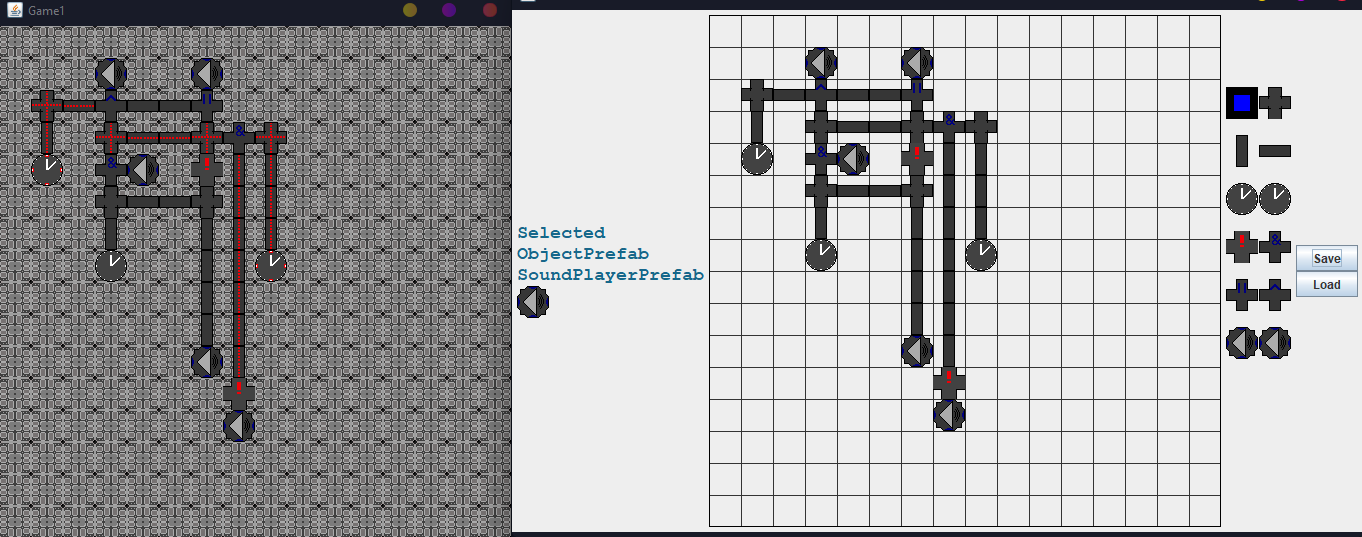
\includegraphics[scale=0.45]{soundboard}
\end{center}
[HEADING SOKOBAN GAME]
One of the requirements of the project was to implement sokoban. We started doing this as soon as there was some resemblance of a framework. Doing this allowed a better understanding of what useful features that the framework would benefit from and shaped large parts of the design. As the framework started to settle in to it’s final version it had changed so much since the work on sokoban started that in order to properly utilize the tools in the framework we chose to create a new version of Sokoban from scratch. Knowing the pitfalls and how to leverage the framework it was a lot less effort and the code was much more presentable.
\\ \\
Our Sokoban also uses the map editor if someone wants to create a map, otherwise there are preloaded maps (if the serialized version did not change, in that case new ones need to be created). Usage of the user input is one of the central parts of sokoban and this displays how the KeyboardInput and the UserInputManager works. In sokoban there is also another interesting detail. That is how multiple objects can exist on one cell, this is done by having an component in one of the gameobjects that is loaded with another gameobject and the unloaded when it is exited. This can in some cases be somewhat unintuitive since the loaded object still thinks that it is in the grid while the grid can only the object in which it is loaded.
Here is an image of the game in action:
\begin{center}
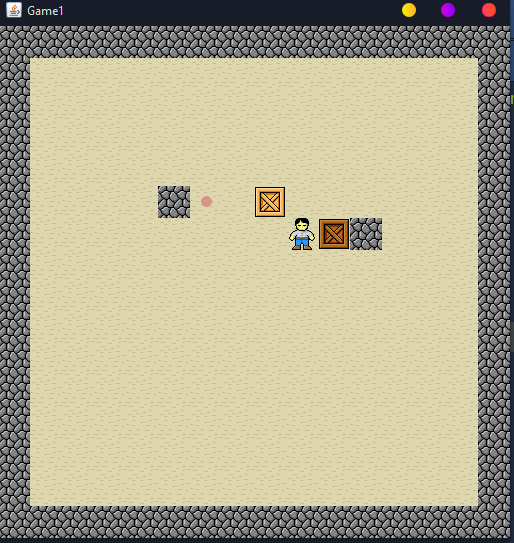
\includegraphics[scale=0.75]{sokoban}
\end{center}
\end{document}